\documentclass[11pt]{article}

\usepackage[margin=1in]{geometry}
\usepackage{graphicx}
\usepackage{array}
\usepackage{multicol}
\usepackage{longtable}
\usepackage{titlesec}
\usepackage{hyperref}
\usepackage{xcolor}
\usepackage{listings}
\usepackage{enumitem}
\usepackage{booktabs}
\usepackage{float}

\lstset{
    basicstyle=\ttfamily\footnotesize,
    breaklines=true,
    frame=single,
    backgroundcolor=\color{gray!10},
    keywordstyle=\color{blue},
    commentstyle=\color{gray},
    stringstyle=\color{orange},
    showstringspaces=false,
    language=Python
}

% Remove extra spacing in lists
\setlist{nosep}
\setlength{\parindent}{0pt}

\title{
    \textbf{Experiment 1: Exploration of Python Libraries} \\
    \large Sri Sivasubramaniya Nadar College of Engineering, Chennai \\
    \normalsize (An Autonomous Institution Affiliated to Anna University)
}
\author{Sreenethi G S}
\date{July 2025}

\begin{document}

\maketitle

\begin{table}[H]
\renewcommand{\arraystretch}{1.5}
\resizebox{\textwidth}{!}{%
\begin{tabular}{|p{5cm}|p{5cm}|p{4cm}|p{3cm}|}
\hline
\textbf{Degree \& Branch}     & B.E. Computer Science \& Engineering & \textbf{Semester} & V \\ \hline
\textbf{Subject Code \& Name} & \multicolumn{3}{c|}{ICS1512 \& Machine Learning Algorithms Laboratory} \\ \hline
\textbf{Academic Year}        & 2025-2026 (Odd) & Batch: 2023–2028 & \textbf{Due Date:} \\ \hline
\end{tabular}
}
\end{table}

\textbf{Aim:} To explore and understand the core functions and methods of Python libraries NumPy, Pandas, SciPy, Scikit-learn, and Matplotlib by performing array manipulations, data preprocessing, mathematical computing, machine learning workflows, and data visualization. To study public datasets, identify appropriate machine learning tasks, and apply the ML workflow steps including feature selection and model evaluation.

\vspace{0.3cm}
\textbf{Libraries Used:} NumPy, Pandas, SciPy, Scikit-learn, Matplotlib, Public Datasets.

\vspace{0.5cm}
\section*{1. Exploration of Python Libraries}

\subsection*{--- NumPy ---}
\textbf{Used for:} Efficient numerical computations, multi-dimensional arrays.
\begin{lstlisting}
import numpy as np

a = np.array([[1, 2], [3, 4]])
b = np.ones((2, 2))

sum_ab = a + b
product = np.dot(a, b)
transpose = a.T

print("Original Array:\n", a)
print("Ones Array:\n", b)
print("Sum:\n", sum_ab)
print("Dot Product:\n", product)
print("Transpose:\n", transpose)
\end{lstlisting}

\begin{figure}[H]
    \centering
    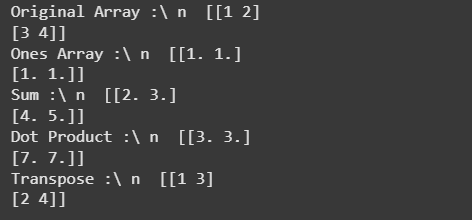
\includegraphics[width=0.8\linewidth]{ml1.png}
    \caption{Output Example 1}
    \label{fig:output1}
\end{figure}

\subsection*{--- Pandas ---}
\textbf{Used for:} Data manipulation and analysis, working with tabular data.
\begin{lstlisting}
import pandas as pd

data = {'Name': ['Alice', 'Bob', 'Charlie'],
        'Age': [25, 30, 35],
        'Score': [85, 90, 95]}
df = pd.DataFrame(data)

df['Passed'] = df['Score'] > 90
mean_score = df['Score'].mean()

print(df)
print("Average Score:", mean_score)
\end{lstlisting}

\begin{figure}[H]
    \centering
    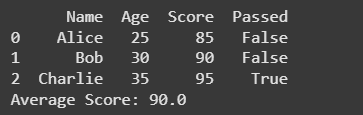
\includegraphics[width=0.8\linewidth]{ml2.png}
    \caption{Output Example 1}
    \label{fig:output1}
\end{figure}

\subsection*{--- SciPy ---}
\textbf{Used for:} Scientific and technical computing (integration, optimization, statistics).
\begin{lstlisting}
from scipy import stats, integrate

group1 = [22, 21, 23, 25, 30]
group2 = [25, 26, 27, 29, 32]
t_stat, p_val = stats.ttest_ind(group1, group2)

area = integrate.quad(lambda x: x**2, 0, 3)[0]

print("T-test p-value:", p_val)
print("Area under x^2 from 0 to 3:", area)
\end{lstlisting}

\begin{figure}[H]
    \centering
    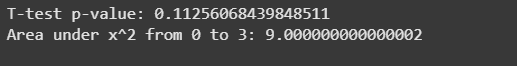
\includegraphics[width=0.8\linewidth]{ml3.png}
    \caption{Output Example 1}
    \label{fig:output1}
\end{figure}

\subsection*{--- Scikit-learn ---}
\textbf{Used for:} Machine learning workflows like preprocessing, training, and evaluation.
\begin{lstlisting}
from sklearn.datasets import load_iris
from sklearn.model_selection import train_test_split
from sklearn.ensemble import RandomForestClassifier
from sklearn.metrics import accuracy_score

iris = load_iris()
X_train, X_test, y_train, y_test = train_test_split(
    iris.data, iris.target, test_size=0.3)

model = RandomForestClassifier()
model.fit(X_train, y_train)

y_pred = model.predict(X_test)
accuracy = accuracy_score(y_test, y_pred)

print("Model Accuracy:", accuracy)
\end{lstlisting}

\begin{figure}[H]
    \centering
    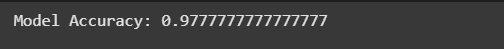
\includegraphics[width=0.8\linewidth]{ml4.png}
    \caption{Output Example 1}
    \label{fig:output1}
\end{figure}

\subsection*{--- Matplotlib ---}
\textbf{Used for:} Data visualization.
\begin{lstlisting}
import matplotlib.pyplot as plt

x = [0, 1, 2, 3, 4]
y = [i**2 for i in x]

plt.plot(x, y, label='y = x^2', color='blue', marker='o')
plt.title("Simple Line Plot")
plt.xlabel("X-axis")
plt.ylabel("Y-axis")
plt.legend()
plt.grid(True)
plt.show()
\end{lstlisting}

\begin{figure}[H]
    \centering
    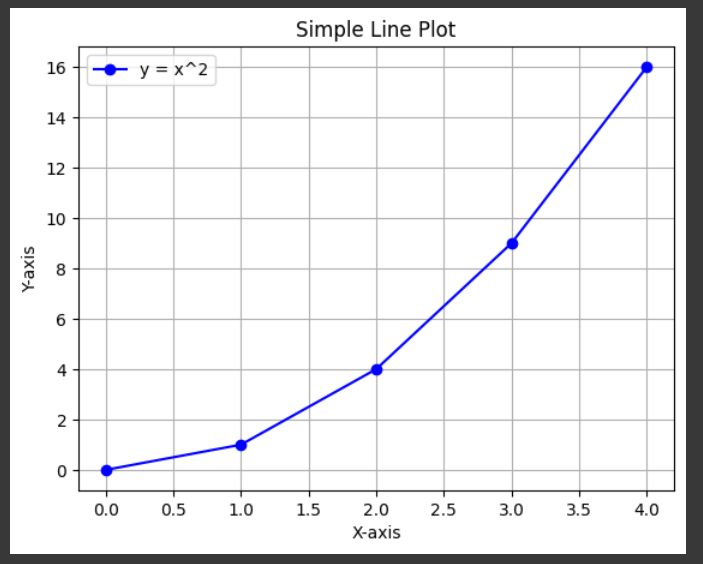
\includegraphics[width=0.8\linewidth]{ml5.png}
    \caption{Output Example 1}
    \label{fig:output1}
\end{figure}

\vspace{0.5cm}
\section*{2. Exploration of Public Datasets and ML Model Type Identification}

\begin{itemize}
    \item \textbf{i) Loan Amount Prediction}  
    \textit{Source:} Kaggle  
    \textit{ML Task:} Supervised – Regression / Classification
    
    \item \textbf{ii) Handwritten Character Recognition}  
    \textit{Source:} UCI / Kaggle  
    \textit{ML Task:} Supervised – Multi-class Classification

    \item \textbf{iii) Email Spam and MNIST Classification}  
    \textit{Source:} UCI (Spam), Kaggle (MNIST)  
    \textit{ML Task:} Supervised – Binary / Multi-class Classification

    \item \textbf{iv) Predicting Diabetes}  
    \textit{Source:} UCI (Pima)  
    \textit{ML Task:} Supervised – Binary Classification

    \item \textbf{v) Iris Dataset}  
    \textit{Source:} UCI  
    \textit{ML Task:} Supervised – Multi-class Classification
\end{itemize}

\section*{3. Machine Learning Workflow and Task Identification}

\subsection*{Types of Machine Learning Tasks}
\begin{table}[h!]
\centering
\renewcommand{\arraystretch}{1.3}
\begin{tabular}{|p{4cm}|p{4cm}|p{6cm}|}
\hline
\textbf{Dataset Example} & \textbf{ML Task Type} & \textbf{Description} \\
\hline
House Price Prediction & Supervised – Regression & Predicts continuous value like price. \\
Email Spam Detection & Supervised – Classification & Classifies emails as spam or not spam. \\
Customer Segmentation & Unsupervised – Clustering & Groups similar users based on features. \\
Movie Recommendation & Unsupervised – Association & Finds items that are bought/watched together. \\
Stock Forecasting & Supervised – Time Series & Predicts future stock values using past data. \\
\hline
\end{tabular}
\end{table}

\subsection*{Machine Learning Workflow Steps}
\begin{enumerate}[label=\roman*.]
    \item \textbf{Loading the Dataset:} Using libraries like \texttt{pandas} or \texttt{NumPy}.
    \item \textbf{Exploratory Data Analysis (EDA):}
    \begin{itemize}
        \item Summary: \texttt{.describe()}, \texttt{.info()}
        \item Plots: Histogram, Boxplot, Heatmap
    \end{itemize}
    \item \textbf{Data Preprocessing:}
    \begin{itemize}
        \item Handle missing values, encode categories, normalize features
    \end{itemize}
    \item \textbf{Feature Selection:}
    \begin{itemize}
        \item Use \texttt{SelectKBest}, Chi-square, or ANOVA F-test
    \end{itemize}
    \item \textbf{Data Splitting:}
    \begin{itemize}
        \item Train/Test split, e.g., 70\% train and 30\% test
    \end{itemize}
    \item \textbf{Performance Evaluation:}
    \begin{itemize}
        \item Classification: Accuracy, F1-score; Regression: RMSE, R\textsuperscript{2}
        \item Clustering: Silhouette Score
    \end{itemize}
\end{enumerate}

\section*{4. Example Dataset-based Tasks}

\begin{table}[h!]
\centering
\renewcommand{\arraystretch}{1.3}
\begin{tabular}{|c|c|c|c|}
\hline
\textbf{Dataset} & \textbf{Type of ML Task} & \textbf{Feature Selection} & \textbf{Suggested Algorithm} \\
\hline
Iris & Classification & All features & Logistic Regression \\
Loan Prediction & Regression / Classification & Income, Credit, Education & Decision Tree \\
Diabetes Prediction & Classification & Glucose, BMI, Age & Random Forest \\
Email Spam Detection & Classification & Word frequencies & Naive Bayes \\
MNIST Digits & Classification & Pixel Intensities & SVM / CNN \\
\hline
\end{tabular}
\end{table}

\section*{5. Results and Discussions}

\begin{itemize}
    \item Successfully explored core Python libraries (NumPy, Pandas, SciPy, Scikit-learn, Matplotlib) for data handling, statistical computing, and machine learning.
    \item Implemented machine learning models like Random Forest on the Iris dataset and evaluated performance using accuracy metrics.
    \item Visualized trends using plots such as line charts and histograms to enhance understanding of data distribution.
    \item Identified suitable ML task types (classification, regression, clustering) for various public datasets.
    \item Applied all stages of a machine learning workflow: loading, EDA, preprocessing, feature selection, model building, and evaluation.
\end{itemize}


\section*{6. Learning Practices}
I learned how to:
\begin{itemize}
    \item Use Python libraries (NumPy, Pandas, SciPy, Scikit-learn, Matplotlib) effectively.
    \item Load and preprocess real-world datasets.
    \item Apply supervised learning algorithms for classification and regression tasks.
    \item Visualize data and model performance.
\end{itemize}

\end{document}
